\subsection{Distribution, suburbs and time}

Prices are heavily right-skewed, yet near-symmetric on a log axis
(Figure~\ref{fig:dist}). This implies the price effects are
multiplicative, and thus, the price target is logarithmically scaled in the modelling pipeline. Dispersion grows with
level, Mosman's standard deviation (\$2.12M) is over six times Blacktown's (\$334k); however,
extreme values are a property of the market, not outliers.

\begin{figure}[H]
\centering
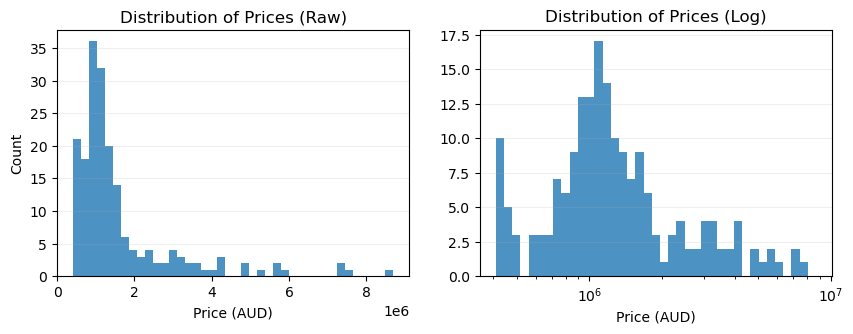
\includegraphics[width=0.86\textwidth]{figures/p2_price_dist.png}\\[1.4ex]
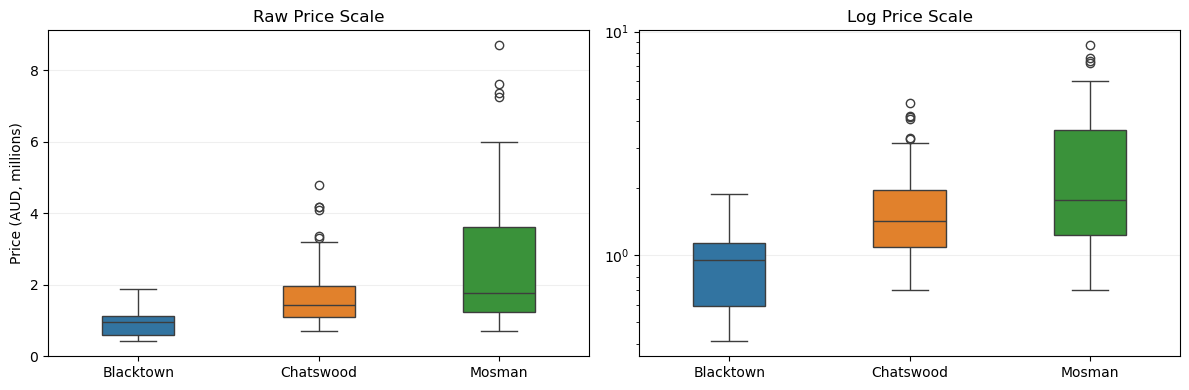
\includegraphics[width=0.86\textwidth]{figures/p2_suburb_box.png}
\caption{Price distribution in raw and log scale (top); by suburb, raw and log scale (bottom).}
\label{fig:dist}
\end{figure}

The temporal view is least trustworthy, across six months, badly unbalanced monthly coverage,
and no repeated seasonal cycle (Figure~\ref{fig:trend}). The correlation heatmap
(Figure~\ref{fig:corr}) shows the SEIFA block is redundant with suburb.

\begin{figure}[H]
\centering
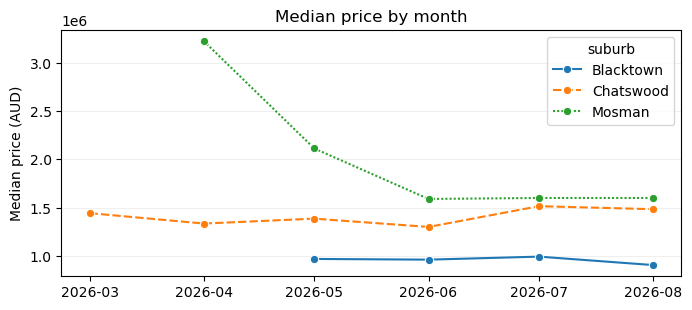
\includegraphics[width=0.72\textwidth]{figures/p2_time_trend.png}
\caption{Median price by month. Coverage is uneven: Blacktown contributes no sales
before May, Chatswood only two in August.}
\label{fig:trend}
\end{figure}

\begin{figure}[H]
\centering
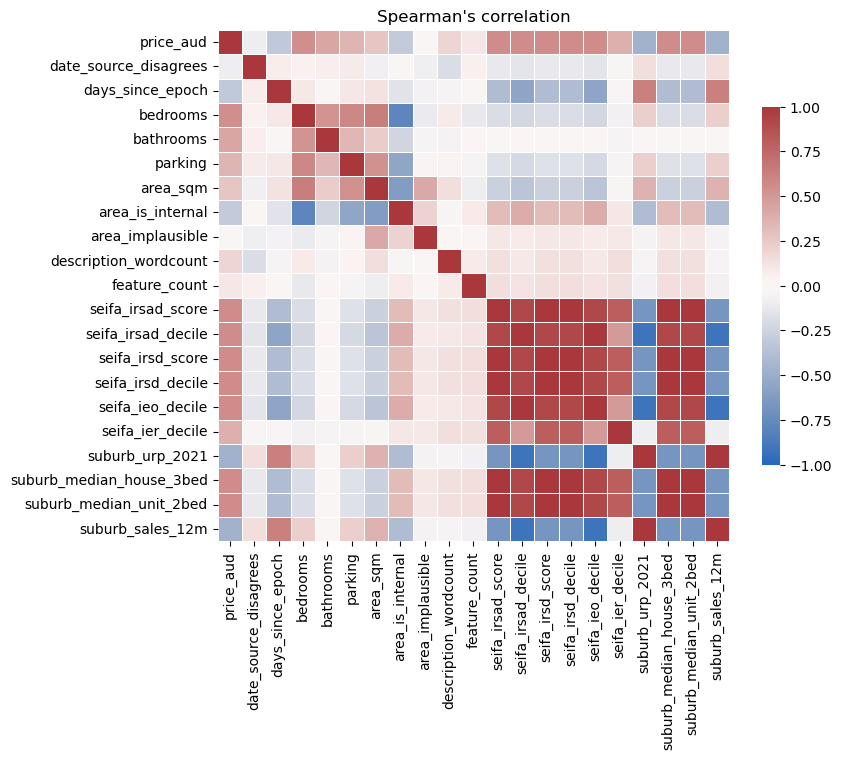
\includegraphics[width=0.55\textwidth]{figures/p2_corr_heatmap.png}
\caption{Spearman $\rho$ correlation, target included. The ten SEIFA and
\texttt{suburb\_*} columns take only three distinct rows, one per suburb, and are
mutually correlated at $\approx 1$.}
\label{fig:corr}
\end{figure}

\begin{figure}[H]
\centering
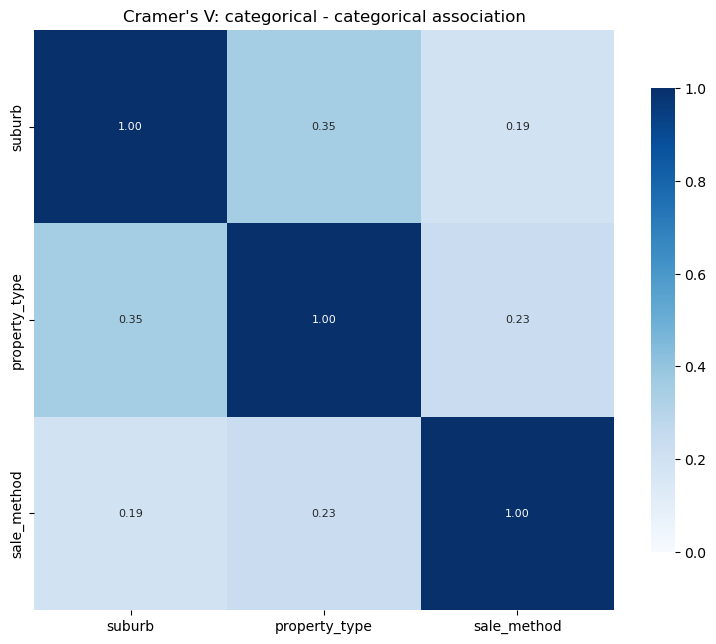
\includegraphics[width=0.35\textwidth]{figures/p2_cramer.png}
\caption{Cramer's $V$ correlation, target excluded}
\label{fig:cramer}
\end{figure}

\subsection{Expected drivers and engineered features}

Three variables were nominated beforehand as most influential, i.e. \textbf{suburb}
(location dominated every comparison above), \textbf{property\_type} (houses and units
priced by different logic) and \textbf{price tercile} (to expose whether accuracy
depends on position in the price range). From these, \texttt{is\_unit} collapses six
types into a land-versus-strata binary, avoiding near-empty categories such as Villa
($n=1$); \texttt{bed\_bath} and \texttt{beds\_x\_unit} summarise size and let a
bedroom's value differ by type, \texttt{t} and \texttt{month} carry time, six
\texttt{kw\_*} flags recover condition signals from agent text.

Remarkably, only two of three survive as inputs, since the price tercile is derived from the target, which leaks a lot of information to the model.
Thus, it serves diagnosis but is never available at prediction time, a limitation of the guess rather than the engineering.
The third nominated driver, size, is measured two ways, i.e. directly by \texttt{area\_sqm}, and indirectly by the room-count composites.
The feature set therefore encodes the intended understanding (location first, type second, size third), though the direct size (\texttt{area\_sqm}) measurement rests on imputation for a third of the sample.
